%
% Soluciones a los ejercicios de Probabilidad II.
%
% Curso 2014 - 2015 2º cuatrimestre
%

%%%%%%%%%%%%%%%%%%%%%%%%%%%%%%%%%%%%%%%%%%%%%%%%%%%%%%%%%%%%%%%%%%%%%%%%%%%%%%%
\section{Hoja 1}

Se asume siempre que estamos trabajando en un espacio de probabilidad $(\Omega, \mathcal{A}, P)$, y que  $\mathcal{B}\subset \mathcal{A}$ es una sub-$\sigma$-\'algebra.

%%%%%%%%%%%%%%%%%%  PROBLEMA 1.1  %%%%%%%%%%%%%%%%%%%%%%%%%
\begin{problem}[1]De una urna con 10 bolas blancas y 10 bolas negras se extraen simultaneamente 3 bolas. 
Calcular la probabilidad de que exactamente dos de ellas sean blancas. Responder a la misma
pregunta si las bolas se extraen de manera sucesiva.
\solution

\begin{expla}
En este caso no hay reposición de las bolas extraídas. Por tanto no hay diferencia a la hora de calcular la probabilidad entre la extracción simultánea y la sucesiva.
\end{expla}
A = Extracción simultánea de 3 bolas blancas

b = blanca

n = negra
\[
P(A)=\underbrace{\frac{10}{20}}_{b}\underbrace{\frac{9}{19}}_{b}\underbrace{\frac{10}{18}}_{n}+\underbrace{\frac{10}{20}}_{b}\underbrace{\frac{10}{19}}_{n}\underbrace{\frac{9}{18}}_{b}+\underbrace{\frac{10}{20}}_{n}\underbrace{\frac{10}{19}}_{b}\underbrace{\frac{9}{18}}_{b} = 3\frac{900}{6840}=\frac{2700}{6840}=0.39
\]

\end{problem}
%%%%%%%%%%%%%%%%%%%%%%%%%%%%%%%%%%%%%%%%%%%%%%%%%%%%%%%%%%


%%%%%%%%%%%%%%%%%%  PROBLEMA 1.2  %%%%%%%%%%%%%%%%%%%%%%%%%
\begin{problem}[2]Disponemos de dos urnas,
$U_1$, que contiene 6 bolas azules y 8 bolas blancas, y
$U_2$,
 que contiene
3 bolas azules y 9 bolas blancas. Se sortea con un dado equilibrado de 4 caras la elecci\'on de una
urna, escogiendose
$U_1$,
si salen 1,
2 o 3, y
$U_2$,
si sale 4. Posteriormente se extrae al azar una bola de
esa urna.

\ppart ?` Cual es la probabilidad de que la bola extraida sea azul?
Sugerencia: usar la regla de la probabilidad total. Respuesta: $43/112$.

\ppart  Si la bola extraida resulta ser blanca  ?`cual es la probabilidad de que proceda de la
urna
$U_1$?

Sugerencia: usar  Bayes o el apartado anterior. Respuesta:
$16/23 = 1 -  43/112$.
\solution
\begin{expla}

$U_1 \rightarrow$ 6a, 8b  (1,2,3)

$U_2 \rightarrow$ 3a, 9b  (4)
\end{expla}
\spart
A = bola extraída azul

$U_1$ = Extraemos de la urna 1

$U_2$ = Extraemos de la urna 2
\[
P(A) = P(A\cap U_1)+P(A\cap U_2) = P(A|U_1)P(U_1)+P(A|U_2)P(U_2)=
\]
\[
=\frac{3}{4}\cdot\frac{6}{14}+\frac{1}{4}\cdot\frac{3}{12}=\frac{18}{56}+\frac{3}{48}=\frac{18}{56}+\frac{1}{16}=\frac{36}{112}+\frac{7}{112}=\frac{43}{112}
\]

\spart
B = bola extraida blanca.

$U_1$ = Extraemos de la urna 1.

\[
P(U_1|B)= \frac{P(U_1 \cap B)}{P(B)} = \frac{P(B|U_1)P(U_1)}{P(B|U_1)P(U_1)+P(B|U_2)P(U_2)}=
\]
\[
=\frac{\frac{8}{14}\cdot\frac{3}{4}}{\frac{8}{14}\cdot\frac{3}{4}+\frac{9}{12}\cdot\frac{1}{4}}=\frac{\frac{24}{56}}{\frac{24}{56}+\frac{9}{48}}=\frac{\frac{24}{56}}{\frac{48}{112}+\frac{21}{112}}=\frac{\frac{24}{56}}{\frac{69}{112}}=\frac{48}{69}=\frac{16}{23}
\]

\end{problem}

%%%%%%%%%%%%%%%%%%%%%%%%%%%%%%%%%%%%%%%%%%%%%%%%%%%%%%%%%%

%%%%%%%%%%%%%%%%%%  PROBLEMA 1.3  %%%%%%%%%%%%%%%%%%%%%%%%%
\begin{problem}[3]Enfermedades raras. Ning\'un test biol\'ogico es 100 $\%$ preciso. Supongamos que un test para
determinar si cierta infecci\'on se ha producido, da falsos positivos en un 1 $\%$ de los casos, y falsos
negativos en un 2 $\%$  de los casos. Si una de cada 100 000 personas entre la poblaci\'on general est\'a
infectada, determinar la probabilidad de que una persona escogida al azar est\'e infectada, sabiendo
que el test ha dado positivo.
\solution

\begin{expla}

\begin{center}
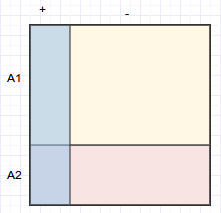
\includegraphics[scale=0.75]{img/Dvenn5.png}
\end{center}


\begin{itemize}

\item Las personas o están infectadas o no están infectadas. 1=P(A1)+P(A2)

\item Los tests o dan positivo o dan negativo: 1 = P(+)+P(-)

\item $A_1$ = persona infectada $\rightarrow P(A1)=10^{-5}$

\item $A_2$ = persona no infectada $\rightarrow P(A_2)=1-10^{-5}$

\item + = test positivo

\item - = test negativo

\item Falso positivo (probabilidad de que el test de positivo estando la persona sin infectar) = $1\% = P(+|A_2)=0.01$

\item $P(+|A_2)+P(-|A_2)=1 \rightarrow P(-|A_2)=0.99$

\item Falso negativo (probabilidad de que el test de negativo sabiendo que la persona esta infectada) = $2\% = P(-|A_1)=0.02$

\item $P(-|A_1)+P(+|A_1)=1 \rightarrow P(+|A_1)=0.98$
\end{itemize}

\end{expla}



\[
P(A_1|+)=\frac{P(A_1\cap B)}{P(+)}=\frac{P(+|A_1)P(A_1)}{P(+|A_1)P(A_1)+P(+|A_2)P(A_2)}=
\]
\[
=\frac{0.98\cdot10^{-5}}{0.98\cdot10^{-5}+0.01\cdot\frac{99999}{10^5}}=0.000979
\]

\end{problem}

%%%%%%%%%%%%%%%%%%%%%%%%%%%%%%%%%%%%%%%%%%%%%%%%%%%%%%%%%%

%%%%%%%%%%%%%%%%%%  PROBLEMA 1.4  %%%%%%%%%%%%%%%%%%%%%%%%%
\begin{problem}[4]Angel y Benito tienen sendas barajas espa\~nolas (40 cartas). Cada uno saca de su
baraja una carta al azar (es decir, con iguales probabilidades, e independientemente). Hallar:

\ppart La probabilidad de obtener al menos un as. 

\ppart La probabilidad de obtener dos cartas del mismo palo. 

\ppart La probabilidad de no obtener ning\'un as.

\ppart La probabilidad de no obtener ni una copa ni una espada.
\solution

\begin{expla}

\end{expla}

\spart
A = obtener al menos un AS

B = no obtener ningun AS
\[
P(A)=\frac{4}{40}\cdot\frac{4}{40}+\frac{4}{40}\cdot\frac{36}{40}+\frac{36}{40}\cdot\frac{4}{40} = 0.19
\]

Otra forma
\[
P(A)=1-P(B)=1-\frac{36}{40}\cdot\frac{36}{40} = 1 - 0.81 = 0.19
\]

\spart
C = dos cartas del mismo palo

Da igual de que palo sea la primera carta, la cosa es que la segunda sea del mismo.

Pensando de otra forma tenemos el siguiente espacio muestral:

$\Omega = \{(c, o),(c, e),(c, b),(c, c),(o, o),(o, c),(o, e),(o, b),(e, c),(e, o),(e, b),(e, e),(b, c),(b, e)\\,(b, o),(b, b)\}$

\[
p(C)=\frac{1}{4}
\]

\spart
B = no obtener ningun AS

\[
P(B)=\frac{36}{40}\cdot\frac{36}{40} = 0.81
\]

\spart
D = no obtener ni una copa ni una espada

\[
P(D) = \frac{20}{40}\cdot\frac{20}{40}=\frac{1}{4}
\]


\end{problem}

%%%%%%%%%%%%%%%%%%%%%%%%%%%%%%%%%%%%%%%%%%%%%%%%%%%%%%%%%%

%%%%%%%%%%%%%%%%%%  PROBLEMA 1.5  %%%%%%%%%%%%%%%%%%%%%%%%%
\begin{problem}[5] Ana y Bea eligen cada una un n\'umero al azar, entre 0 y 2. Sean $A, B, C, D,$ los siguientes
eventos: 

\  $A$: La diferencia entre ambos n\'umeros es al menos 1/3.

\ $B$:   Al menos uno de los n\'umeros es mayor que 1/3.

\ $C$: Los dos n\'umeros son iguales.

\ $D$: El n\'umero de Bea es mayor que 1/3.

Hallar $P(B)$, $P(C)$ y $P(A\cup D)$.
\solution

\begin{expla}
Suponemos que el número elegido es natural, es decir, pertenece al conjunto $\{0,1,2\}$.
\end{expla}

\spart
E = Ningún número es mayor que 1/3.

\[
P(B)=1 - P(E)= 1 - \frac{1}{3}\cdot\frac{1}{3} = \frac{8}{9}
\]

\spart

Da igual qué numero escojas el primero, el que importa es el segundo.

Pensando de otra forma tenemos el siguiente espacio muestral:

$\Omega=\{(0,0),(0,1),(0,2),(1,0),(1,1),(1,2),(2,0),(2,1),(2,2)\}$

\[
P(C)=\frac{1}{3}
\]

\spart
Dado el espacio muestral $\Omega$ definido en el apartado anterior, vemos que:

$P(A)=\frac{2}{3}$ 

Ya que los elementos que cumplen A son: \{(0,1),(0,2),(1,0),(1,2),(2,0),(2,1)\}

$P(D)=\frac{2}{3}$

Ya que los elementos que cumplen D son: \{(0,1),(0,2),(1,1),(1,2),(2,1),(2,2)\}

Por tanto, los elementos que cumplen $A\cup D$ serán la unión de los elementos que cumplen A y los que cumplen D.

\[
P(A \cup D) = \frac{8}{9}
\]

\end{problem}

%%%%%%%%%%%%%%%%%%%%%%%%%%%%%%%%%%%%%%%%%%%%%%%%%%%%%%%%%%

%%%%%%%%%%%%%%%%%%  PROBLEMA 1.6  %%%%%%%%%%%%%%%%%%%%%%%%%
\begin{problem}[6]Con 12 chicas y 4 chicos se forman al azar 4 grupos de 4 personas.
Calcular la probabididad de que haya un chico en cada grupo. Sugerencia:
usar la regla del producto.
 
\solution

\begin{expla}

$A_n$ = Un chico en el grupo n

B = Un chico en cada grupo
\end{expla}

$P(A_1)=4\cdot\frac{4}{16}\cdot\frac{12}{15}\cdot\frac{11}{14}\cdot\frac{10}{13}=0.4835$

$P(A_2|A_1)=4\cdot\frac{3}{12}\cdot\frac{9}{11}\cdot\frac{8}{10}\cdot\frac{7}{9}=0.509$

$P(A_3|A_1\cap A_2)=4\cdot\frac{2}{8}\cdot\frac{6}{7}\cdot\frac{5}{6}\cdot\frac{4}{5}=0.5714$

$P(A_4|A_1\cap A_2\cap A_3)=4\cdot\frac{1}{4}\cdot\frac{3}{3}\cdot\frac{2}{2}\cdot\frac{1}{1}=1$


\[
P(B)=\bigcap_{n=1}^4P(A_n)=P(A_1)P(A_2|A_1)P(A_3|A_2\cap A_1)P(A_4|A_1\cap A_2\cap A_3)=0.14
\]




\end{problem}

%%%%%%%%%%%%%%%%%%%%%%%%%%%%%%%%%%%%%%%%%%%%%%%%%%%%%%%%%%

%%%%%%%%%%%%%%%%%%  PROBLEMA 1.7  %%%%%%%%%%%%%%%%%%%%%%%%%
\begin{problem}[7]Benito tiene un dado  trucado, con 6 caras  numeradas del 1 al 6. 
La probabilidad de las
distintas caras es proporcional al n\'umero de puntos inscritos en
ellas. Hallar la probabilidad de que Benito obtenga con ese dado un n\'umero
par.
\solution

\begin{expla}

Teniendo en cuenta que la suma de los números del dado es 21

\end{expla}

\[
P(par)=P(2)+P(4)+P(6)=\frac{2}{21}+\frac{4}{21}+\frac{6}{21}=\frac{12}{21}=0.57
\]

\end{problem}

%%%%%%%%%%%%%%%%%%%%%%%%%%%%%%%%%%%%%%%%%%%%%%%%%%%%%%%%%%

%%%%%%%%%%%%%%%%%%  PROBLEMA 1.8  %%%%%%%%%%%%%%%%%%%%%%%%%
\begin{problem}[8] En el esquema que aparece a continuaci\'on, el agua fluye  desde $A$ hacia
$B$. Hay, como se indica en el dibujo, ocho compuertas.
Independientemente unas de otras, cada compuerta est\'{a} abierta con
probabilidad $p$, $0 <p <1$. Calcular la probabilidad de que el agua llegue
 de $A$ a $B$. Calcular dicha probabilidad cuando $p = 1/3$.
% Drawing generated by LaTeX-CAD 1.8a - requires latexcad.sty
% (c) 1996 John Leis leis@usq.edu.au
$$\xymatrix{    &   & \circ\ar @{.}[dr]!U||&  &   \circ  \ar @{.}[dr]!U|| &  &  \\
A \ar[r]  & \circ  \ar @{.}[ru]!U||   \ar @{.}[rd]!U||   & &  \circ \ar @{.}[ru]!U||  \ar @{.}[rd]!U||  & & \circ \ar[r]  & B\\  
  &   & \circ \ar @{.}[ru]!U||  &  &   \circ  \ar @{.}[ru]!U||   &  &  }$$ 

Respuestas: $p^8 - 4 p^6 + 4 p^4, 289/6561$.
\solution

\begin{expla}

\end{expla}

Se entiende que en las intersecciones el agua va en todas las direcciones.

Llamamos C al punto intermedio (a la intersección entre los dos rombos).

Para llegar hasta el punto C, tenemos que considerar la existencia de 4 puertas: $P_1, P_2, P_3, P_4$, enumeradas de izquierda a derecha y de arriba hacia abajo. Por tanto, para que el agua llegue a C, deben estar abiertas al menos $P_1$ y $P_2$, o $P_3$ y $P_4$.

Si consideramos el siguiente espacio muestral:

$\Omega = \{(0000),(0001),(0010),(0011),(0100),(0101),...,(1110),(1111)\}$

Formado por 16 elementos, en los que un 1 en la posición n indica que la puerta $P_n$ está abierta, tenemos que con esas 16 combinaciones el agua NO llegaría a C en los elementos con 4 0's (1), los elementos con 3 0,s (4) y los elementos 1010, 0101, 1001, 0110 (4). Por tanto solo nos sirven 7 combinaciones. La de todo 1's, las de 3 1's (4), 1100 y 0011.

$P(1100)=P(0011)=p^2(1-p)^2$

$P(1110)=P(1101)=P(1011)=P(0111)=p^3(1-p)$

$P(1111)=p^4$

Por tanto la probabilidad de llegar a C desde A es:

\[
P(AC)=2p^2(1-p)^2+4p^3(1-p)+p^4
\]

La probabilidad de llegar al punto B, desde el punto C es exactamente la misma que la de ir desde A hasta C. Por tanto, según la regla del producto quedaría:
\[
P(AB)=P(AC)P(CB|AC)=P(AC)^2=(2p^2(1-p)^2+4p^3(1-p)+p^4)^2=
\]
\[
=(2p^2(p^2+1-2p)+4p^3-4p^4+p^4)^2 = (2p^4 + 2p^2-4p^3-3p^4+4p^3)^2 =
\]
\[
=(-p^4+2p^2)^2=p^8-4p^6+4p^4
\]

Para $p=\frac{1}{3}$, nos queda:

\[
P(AB)=\frac{1}{3^8}-4\cdot\frac{1}{3^6}+4\cdot\frac{1}{3^4}=\frac{289}{6561}
\]



\end{problem}

%%%%%%%%%%%%%%%%%%%%%%%%%%%%%%%%%%%%%%%%%%%%%%%%%%%%%%%%%%

%%%%%%%%%%%%%%%%%%  PROBLEMA 1.9  %%%%%%%%%%%%%%%%%%%%%%%%%
\begin{problem}[9]En una reuni\'on hay 25 personas. Calcular la
probabilidad de que celebren su cumplea\~{n}os el mismo d\'ia del
a\~{n}o al menos dos personas. Observación: con frecuencia es m\'as f\'acil
calcular intersecciones que uniones. Sugerencia: calcular la probabilidad
del evento complementario.
\solution

\begin{expla}

\end{expla}

A = cumpleaños mismo día al menos dos personas.

$A^c$ = cumpleaños distinto día todas las personas.

\[
P(A)=1-P(A^c)=1-\frac{365}{365}\cdot\frac{364}{365}\cdot\frac{363}{365}\cdot...\cdot\frac{341}{365}=1-0.43=0.57
\]

\end{problem}

%%%%%%%%%%%%%%%%%%%%%%%%%%%%%%%%%%%%%%%%%%%%%%%%%%%%%%%%%%

%%%%%%%%%%%%%%%%%%  PROBLEMA 1.10  %%%%%%%%%%%%%%%%%%%%%%%%%
\begin{problem}[10]Inclusi\'on-Exclusi\'on: Probar que 
$
P(\cup_{i=1}^n A_i)= \sum_{k=1}^n \sum_{I\subset \{1, \dots, n\}, |I| = k} (-1)^{k-1}
P(\cap_{i\in I} A_i).
$
\solution

\begin{expla}

Tenemos que probar:

\[
P(\bigcup_{i=1}^nA_i)=\sum_{k=1}^{n}\sum_{I\subset \{1,...,n\}:|I|=k}(-1)^{k-1}P(\bigcap_{i\in I}A_i)
\]

Vamos a ver lo que significa para una colección de 3 subconjuntos $\{A_1,A_2,A_3\}$; de forma que sea fácil de ver. El término que puede llevar a la duda es el segundo sumatorio, sólo dice que escojamos todas las subcolecciones posibles de tamaño k dentro de nuestra colección $\{A_1,A_2,A_3\}$.

\begin{center}
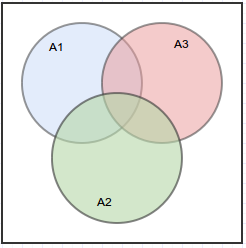
\includegraphics[scale=0.75]{img/Dvenn4.png}
\end{center}

\[
P(A_1\cup A_2 \cup A_3)=\underbrace{(-1)^0P(A_1)+(-1)^0P(A_2)+(-1)^0P(A_3)}_{k=1}+
\]
\[
+\underbrace{(-1)^1P(A_1\cap A_2)+(-1)^1P(A_1\cap A_3)+(-1)^1P(A_2\cap A_3)}_{k=2}+\underbrace{(-1)^2P(A_1\cap A_2\cap A_3)}_{k=3}=
\]
\[
=\underbrace{P(A_1)+P(A_2)+P(A_3)}_{k=1}+\underbrace{(-P(A_1\cap A_2)-P(A_1\cap A_3)-P(A_2\cap A_3))}_{k=2}+\underbrace{P(A_1\cap A_2\cap A_3)}_{k=3}
\]

\end{expla}

Estamos en ello

\end{problem}

%%%%%%%%%%%%%%%%%%%%%%%%%%%%%%%%%%%%%%%%%%%%%%%%%%%%%%%%%%

%%%%%%%%%%%%%%%%%%  PROBLEMA 1.11  %%%%%%%%%%%%%%%%%%%%%%%%%
\begin{problem}[11] Emparejamientos al azar: tenemos $n$ cartas, que colocamos al azar en $n$ sobres
(en vez de cuidadosamente poner cada carta en su sobre).
Calcular la probabilidad de que alguna carta est\'a en el sobre correcto
(es decir, al menos una carta). Estimar dicha probabilidad cuando
$n\to\infty$. Sugerencia: usar Inclusi\'on-Exclusi\'on.
Observar que la probabilidad de que todas las cartas de 1 a $k$ esten en el sobre correcto
es $(n-k)!/n!$. Respuesta en el l\'{\i}mite: $1 - e^{-1}$.
\solution

\begin{expla}

Para hacernos una idea del problema consideramos n=3 y el siguiente espacio de probabilidad:

$\Omega_3=\{(123),(132),(213),(231),(312),(321)\}$

Que representa todas las posibles combinaciones (numero de carta-numero sobre) que puede haber con 3 cartas y 3 sobres. 

Según esto la probabilidad de que la carta 1 este en el sobre 1 sería: $\frac{2}{6} = \frac{2}{3\cdot 2}=\frac{1}{3}$

Sea: $A_i$ = carta n-esima en el sobre correcto.

Se observa fácilmente que: $P(A_i) = \frac{(n-1)!}{n!}$, siendo n el número de cartas totales.

Sea A = todas las cartas en el sobre correcto. Simplemente hay que observar que si la primera carta esta en el sobre correcto, para poner la segunda en su sobre tenemos una carta y un sobre menos donde elegir.

\[
P(A)=P(\bigcap_{j=1}^nA_j)=P(A_1)P(A_2|A_1)P(A_3|A_2\cap A_1)...P(A_j|\bigcap_{i=1}^{n-1}A_i)=
\]
\[
\frac{(n-1)!}{n!}\cdot\frac{(n-2)!}{(n-1)!}\cdot\frac{(n-3)!}{(n-2)!}\cdot...\cdot\frac{(n-n+1)!}{(n-n+2)!}\cdot\frac{(n-n)!}{(n-n+1)!}=\frac{1}{n!}
\]

Sea $B_k$ = todas las cartas de la 1 a la k en el sobre correcto.

\[
P(B_k)=P(\bigcap_{n=1}^kA_n)=P(A_1)P(A_2|A_1)P(A_3|A_2\cap A_1)...P(A_n|\bigcap_{i=1}^{k-1}A_i)=
\]
\[
\frac{(n-1)!}{n!}\cdot\frac{(n-2)!}{(n-1)!}\cdot\frac{(n-3)!}{(n-2)!}\cdot...\cdot\frac{(n-k+1)!}{(n-k+2)!}\cdot\frac{(n-k)!}{(n-k+1)!}=\frac{(n-k)!}{n!}
\]

Esta probabilidad es la misma cojamos las k primeras cartas o k cartas en diferentes posiciones.
\end{expla}

Vamos a usar Inclusión-Exclusión:
\[
P(\bigcup_{i=1}^nA_i)=\sum_{k=1}^{n}\sum_{I\subset \{1,...,n\}:|I|=k}(-1)^{k-1}P(\bigcap_{i\in I}A_i)
\]

C = Al menos una carta en el sobre correcto: 

\[
P(C)=P(\bigcup_{i=1}^nA_i)=\sum_{k=1}^{n}\sum_{I\subset \{1,...,n\}:|I|=k}(-1)^{k-1}\frac{(n-k)!}{n!}=\sum_{k=1}^{n}\left( (-1)^{k-1}\frac{(n-k)!}{n!}\binom{n}{k}\right)=
\]
\[
= \sum_{k=1}^{n}\left( (-1)^{k-1}\frac{(n-k)!}{n!}\cdot \frac{n!}{(n-k)!\cdot k!}\right)= \sum_{k=1}^{n}\left( (-1)^{k-1}\frac{1}{k!}\right) \stackrel{n \rightarrow \infty}{\rightarrow} 1-e^{-1}
\]

\textcolor{red}{El limite es asi porque si, luego busco una demostración de ese límite}



\end{problem}

%%%%%%%%%%%%%%%%%%%%%%%%%%%%%%%%%%%%%%%%%%%%%%%%%%%%%%%%%%

%%%%%%%%%%%%%%%%%%  PROBLEMA 1.12  %%%%%%%%%%%%%%%%%%%%%%%%%
\begin{problem}[12] Media o esperanza. Con los datos del problema anterior, calcular el n\'umero esperado de
emparejamientos al azar, es decir, cuantas cartas esperamos que est\'an en el sobre correcto.
Comentario: este problema es muy f\'acil.
\solution

\begin{expla}

\end{expla}

\end{problem}

%%%%%%%%%%%%%%%%%%%%%%%%%%%%%%%%%%%%%%%%%%%%%%%%%%%%%%%%%%

%%%%%%%%%%%%%%%%%%  PROBLEMA 1.13  %%%%%%%%%%%%%%%%%%%%%%%%%
\begin{problem}[13] Dado $C$ con $P(C) > 0$, decimos que $A$ y $B$ son condicionalmente independientes
con respecto a $C$ si $P(A\cap B|C) =P(A|C) P(B|C)$. Probar que si  $P(B\cap C) > 0$, 
$P(A\cap B|C) =P(A|C) P(B|C)$ es equivalente a $P(A|C) = P(A|B \cap C)$. 


\solution

\begin{expla}

\end{expla}

\end{problem}

%%%%%%%%%%%%%%%%%%%%%%%%%%%%%%%%%%%%%%%%%%%%%%%%%%%%%%%%%%

%%%%%%%%%%%%%%%%%%  PROBLEMA 1.14  %%%%%%%%%%%%%%%%%%%%%%%%%
\begin{problem}[14] Estudiar para $ \alpha>0 $ la convergencia en
media cuadr\'atica (es decir, en $L^2$) de la sucesi\'on $\{X_n\}_{n=1}^\infty$, sabiendo que

\[  P(X_n=n)=\frac{1}{n^\alpha}, \hspace{5mm} P(X_n=0)=1-\frac{1}{n^\alpha}.
  \]
\solution

\begin{expla}

\end{expla}

\end{problem}

%%%%%%%%%%%%%%%%%%%%%%%%%%%%%%%%%%%%%%%%%%%%%%%%%%%%%%%%%%





\newpage
\section{Hoja 2}

Salvo afirmación expresa en sentido contrario se asume siempre que estamos trabajando en un espacio de probabilidad $(\Omega, \mathcal{A}, P)$,
que  $\mathcal{B}\subset \mathcal{A}$ es una sub-$\sigma$-\'algebra, que las funciones son medibles, etc..

Recordatorio: si $1\le p < \infty$, $\|f\|_p := \left(\int|f|^p\right)^{1/p}$, mientras que
$\|f\|_\infty$ denota el supremo esencial de $|f|$. De hecho, la definición
 $\|f\|_p := \left(\int|f|^p\right)^{1/p}$ tiene sentido para cualquier $p > 0$ finito, pero puede
demostrarse que si $p < 1$ esta expresi\'on no define una norma.

%%%%%%%%%%%%%%%%%%  PROBLEMA 2.1  %%%%%%%%%%%%%%%%%%%%%%%%%
\begin{problem}[1]En el esquema que aparece a continuaci\'on, el agua fluye  desde $A$ hacia
$B$. Hay, como se indica en el dibujo, ocho compuertas.
Independientemente unas de otras, cada compuerta est\'{a} abierta con
probabilidad $p$, $0 <p <1$. Calcular la probabilidad de que el agua llegue
 de $A$ a $B$. Calcular dicha probabilidad cuando $p = 1/3$.
% Drawing generated by LaTeX-CAD 1.8a - requires latexcad.sty
% (c) 1996 John Leis leis@usq.edu.au
$$\xymatrix{    &   & \circ\ar @{.}[dr]!U||&  &   \circ  \ar @{.}[dr]!U|| &  &  \\
A \ar[r]  & \circ  \ar @{.}[ru]!U||   \ar @{.}[rd]!U||   & &  \circ \ar @{.}[ru]!U||  \ar @{.}[rd]!U||  & & \circ \ar[r]  & B\\  
  &   & \circ \ar @{.}[ru]!U||  &  &   \circ  \ar @{.}[ru]!U||   &  &  }$$
\solution

\begin{expla}

\end{expla}

\end{problem}
%%%%%%%%%%%%%%%%%%%%%%%%%%%%%%%%%%%%%%%%%%%%%%%%%%%%%%%%%%


%%%%%%%%%%%%%%%%%%  PROBLEMA 2.2  %%%%%%%%%%%%%%%%%%%%%%%%%
\begin{problem}[2]Probar o refutar:
Para toda $X:\Omega \to \mathbb{R}$, $E(X|  \mathcal{A})^+ = E(X^+|  \mathcal{A})$.
\solution

\begin{expla}

\end{expla}

\end{problem}

%%%%%%%%%%%%%%%%%%%%%%%%%%%%%%%%%%%%%%%%%%%%%%%%%%%%%%%%%%

%%%%%%%%%%%%%%%%%%  PROBLEMA 2.3  %%%%%%%%%%%%%%%%%%%%%%%%%
\begin{problem}[3]La desigualdad aritm\'etico-geom\'etrica 
dice que la media  aritm\'etica de un conjunto de n\'umeros no negativos es al menos tan grande
como su media  geom\'etrica, es decir, si $a_1, \dots ,a_n > 0$ satisfacen  $a_1 + \cdots  + a_n = 1$,  y  
 $x_1, \dots ,x_n \ge 0$, entonces $\Pi_{i=1}^n x_i^{a_i} \le \sum_{i=1}^n a_i x_i$.
Demostrar dicha desigualdad. Sugerencia: usar la concavidad
de log, o la convexidad de exp.
\solution

\begin{expla}

\end{expla}

\end{problem}

%%%%%%%%%%%%%%%%%%%%%%%%%%%%%%%%%%%%%%%%%%%%%%%%%%%%%%%%%%

%%%%%%%%%%%%%%%%%%  PROBLEMA 2.4  %%%%%%%%%%%%%%%%%%%%%%%%%
\begin{problem}[4]Demostrar la siguiente desigualdad de Young: para $t, u \ge 0$, y $p,q > 1$ tales que
$1/p + 1/q =1$, tenemos $tu \le t^p/ p + u^q/ q$. Observaci\'on: \'esta es otra forma de
escribir la  desigualdad aritm\'etico-geom\'etrica para $n=2$, mediante un cambio obvio de variables.
\solution

\begin{expla}

\end{expla}

\end{problem}

%%%%%%%%%%%%%%%%%%%%%%%%%%%%%%%%%%%%%%%%%%%%%%%%%%%%%%%%%%

%%%%%%%%%%%%%%%%%%  PROBLEMA 2.5  %%%%%%%%%%%%%%%%%%%%%%%%%
\begin{problem}[5]Sean $p,q \ge 1$ exponentes conjugados, es decir, $p$ y $q$ satisfacen
$1/p + 1/q =1$ (si $p=1$, entonces $q = \infty$, y viceversa).
Dado un espacio de medida arbitrario $(\Omega, \mathcal{A}, \mu)$, demostrar la desigualdad de
H\"older: si $f\in L^p$ y $g\in L^q$, entonces $fg\in L^1$, y $\|fg\|_1 \le \|f\|_p\|g\|_q$.
Sugerencias: El caso $p=1, q=\infty$ sale directamente de las definiciones.
Para $p >1$, suponemos que  $\|f\|_p, \|g\|_q\ne 0$, y reemplazamos 
$f$ y $g$ con 
 $f/\|f\|_p$ y $g/\|g\|_q$.  Despu\'es usamos la desigualdad de Young (punto a
punto) e integramos.
\solution

\begin{expla}

\end{expla}

\end{problem}

%%%%%%%%%%%%%%%%%%%%%%%%%%%%%%%%%%%%%%%%%%%%%%%%%%%%%%%%%%

%%%%%%%%%%%%%%%%%%  PROBLEMA 2.6  %%%%%%%%%%%%%%%%%%%%%%%%%
\begin{problem}[6] Dada $f:\Omega\to \mathbb{R}$ en $L^p$,  $1 < p <  \infty$, escoger $g\in L^q$ tal que
$\int fg = \|fg\|_1 = \|f\|_p\|g\|_q$. Concluir que 
$\|f\|_p= \operatorname{sup}_{\{g\in L^q: \|g\|_q=1\}} \int fg $.
\solution

\begin{expla}

\end{expla}

\end{problem}

%%%%%%%%%%%%%%%%%%%%%%%%%%%%%%%%%%%%%%%%%%%%%%%%%%%%%%%%%%

%%%%%%%%%%%%%%%%%%  PROBLEMA 2.7  %%%%%%%%%%%%%%%%%%%%%%%%%
\begin{problem}[7]Usar $\|f\|_p= \operatorname{sup}_{\{g\in L^q: \|g\|_q=1\}} \int fg $ cuando $1 < p <  \infty$
para obtener la desigualdad triangular o de Minkowski: $\|f + g\|_p \le \|f\|_p + \|g\|_p$.
Probar tambi\'en los casos (bastante obvios) $p=1$  y  $p = \infty$.
\solution

\begin{expla}

\end{expla}

\end{problem}

%%%%%%%%%%%%%%%%%%%%%%%%%%%%%%%%%%%%%%%%%%%%%%%%%%%%%%%%%%

%%%%%%%%%%%%%%%%%%  PROBLEMA 2.8  %%%%%%%%%%%%%%%%%%%%%%%%%
\begin{problem}[8]Probar que $\|\cdot\|_p$ es una norma en $L^p$ (considerando que dos funciones
son iguales
cuando son iguales en casi todo punto).
\solution

\begin{expla}

\end{expla}

\end{problem}

%%%%%%%%%%%%%%%%%%%%%%%%%%%%%%%%%%%%%%%%%%%%%%%%%%%%%%%%%%

%%%%%%%%%%%%%%%%%%  PROBLEMA 2.9  %%%%%%%%%%%%%%%%%%%%%%%%%
\begin{problem}[9]Probar la desigualdad de Jensen: si $X:\Omega\to I\subset \mathbb{R}$, donde
$I$ es un intervalo en $\mathbb{R}$, y $X$ tiene media finita, entonces para toda funci\'on
convexa $g:I\to \mathbb{R}$, $g(EX) \le E(g(X))$. Comentario: el caso particular $g(t) = t^2$
ya se ha visto (y usado) en clase. Es consecuencia de la no negatividad de la varianza.
Sugerencia: si $L(t) := a t + b$ es una recta, entonces conmuta con la integraci\'on:
$L(\int X(\omega) dP (\omega)) = \int L (X(\omega)) dP (\omega)$. La desigualdad de Jensen
es consecuencia de esta observaci\'on, junto con el hecho de que las funciones convexas
est\'an por encima de todas sus rectas soporte.
\solution

\begin{expla}

\end{expla}

\end{problem}

%%%%%%%%%%%%%%%%%%%%%%%%%%%%%%%%%%%%%%%%%%%%%%%%%%%%%%%%%%

%%%%%%%%%%%%%%%%%%  PROBLEMA 2.10  %%%%%%%%%%%%%%%%%%%%%%%%%
\begin{problem}[10]Probar que si $0 < r\le s \le \infty$,
 entonces $\|f\|_{L^r(\Omega, \mathcal{A}, P)}\le \|f\|_{L^s(\Omega, \mathcal{A}, P)}$, luego $L^s(\Omega, \mathcal{A}, P) \subset L^r(\Omega, \mathcal{A}, P)$ (sugerencia, usar Jensen o H\"older). Demostrar que si el espacio tiene medida infinita, esta
inclusi\'on puede fallar.
\solution

\begin{expla}

\end{expla}

\end{problem}

%%%%%%%%%%%%%%%%%%%%%%%%%%%%%%%%%%%%%%%%%%%%%%%%%%%%%%%%%%


\newpage
\section{Hoja 3}

Salvo afirmaci\'on expresa en sentido
contrario se asume siempre que estamos trabajando en un espacio de probabilidad $(\Omega, \mathcal{A}, P)$,
que  $\mathcal{B}\subset \mathcal{A}$ es una sub-$\sigma$-\'algebra, que las funciones son medibles, etc..


Recordatorio: si $1\le p < \infty$, $\|f\|_p := \left(\int|f|^p\right)^{1/p}$, mientras que
$\|f\|_\infty$ denota el supremo esencial de $|f|$. \

%%%%%%%%%%%%%%%%%%  PROBLEMA 3.1  %%%%%%%%%%%%%%%%%%%%%%%%%
\begin{problem}[1] Pepe y Jaime juegan con una moneda equilibrada, lanz\'andola hasta que por primera vez 
aparece la sucesi\'on  de longitud dos  elegida por uno de ellos. Usamos 1 para representar
cara, 0 para representar cruz.
Pepe escoge la sucesi\'on 11, y a continuaci\'on, Jaime elige  01, pensando que ello le da ventaja. 
Hallar la probabilidad de que gane Jaime.
\solution

\begin{expla}

\end{expla}

\end{problem}
%%%%%%%%%%%%%%%%%%%%%%%%%%%%%%%%%%%%%%%%%%%%%%%%%%%%%%%%%%


%%%%%%%%%%%%%%%%%%  PROBLEMA 3.2  %%%%%%%%%%%%%%%%%%%%%%%%%
\begin{problem}[2] Probar que si $X := \{X_n\}_{n=0}^{\infty}$  es una martingala adaptada a la filtraci\'on
$\{\mathcal{A}_n\}_{n=0}^{\infty}$, entonces para todo $n>0$ tenemos 
$EX_n = EX_0$. 
Enunciar los resultados an\'alogos para sub y supermartingalas.
\solution

\begin{expla}

\end{expla}

\end{problem}

%%%%%%%%%%%%%%%%%%%%%%%%%%%%%%%%%%%%%%%%%%%%%%%%%%%%%%%%%%

%%%%%%%%%%%%%%%%%%  PROBLEMA 3.3  %%%%%%%%%%%%%%%%%%%%%%%%%
\begin{problem}[3] Probar que si $X := \{X_n\}_{n=0}^{\infty}$  es una martingala adaptada a la filtraci\'on
$\{\mathcal{A}_n\}_{n=0}^{\infty}$, entonces para todo $m, n\ge 0$ tenemos
$E(X_{n + m}|\mathcal{A}_n) = X_n$. Enunciar los resultados an\'alogos para sub y supermartingalas.
\solution

\begin{expla}

\end{expla}

\end{problem}

%%%%%%%%%%%%%%%%%%%%%%%%%%%%%%%%%%%%%%%%%%%%%%%%%%%%%%%%%%

%%%%%%%%%%%%%%%%%%  PROBLEMA 3.4  %%%%%%%%%%%%%%%%%%%%%%%%%
\begin{problem}[4] Sea $\{X_n\}_{n=0}^{\infty}$ una sucesi\'on de v.a.i.i.d., tales que 
$P(X_i = 1)= P(X_i = -1) = 1/2$, y sea $S_n := \sum_{i=0}^n X_i$.
Probar que $S := \{S_n\}_{n=0}^{\infty}$  es una martingala adaptada a la filtraci\'on
$\{\mathcal{A}_n\}_{n=0}^{\infty}$, donde $\mathcal{A}_n := \sigma(X_0, \dots, X_n)$.
En la demostraci\'on puede usarse el hecho de que si la v.a. $Y$ es independiente
de la $\sigma$-\'algebra $\mathcal{B}$, entonces $E(Y|\mathcal{B}) = E(Y)$.
\solution

\begin{expla}

\end{expla}

\end{problem}

%%%%%%%%%%%%%%%%%%%%%%%%%%%%%%%%%%%%%%%%%%%%%%%%%%%%%%%%%%

%%%%%%%%%%%%%%%%%%  PROBLEMA 3.5  %%%%%%%%%%%%%%%%%%%%%%%%%
\begin{problem}[5] C\'omo ganar un euro con probabilidad 1, en un juego justo: la estrat\'egia del doble o nada.
Apostamos un euro a que sale cara. Si sale cara nos plantamos, si sale cruz apostamos
2 euros a que sale cara. Si sale cara nos plantamos, si sale cruz apostamos
4 euros a que sale cara. Etc.. Demostrar que la  estrat\'egia anterior gana un euro
 con probabilidad 1.
\solution

\begin{expla}

\end{expla}

\end{problem}

%%%%%%%%%%%%%%%%%%%%%%%%%%%%%%%%%%%%%%%%%%%%%%%%%%%%%%%%%%



\newpage
\section{Hoja 4}

Salvo afirmaci\'on expresa en sentido
contrario se asume siempre que estamos trabajando en un espacio de probabilidad $(\Omega, \mathcal{A}, P)$,
que  $\mathcal{B}\subset \mathcal{A}$ es una sub-$\sigma$-\'algebra, que las funciones son medibles, etc..

Recordatorio: si $0 < p < \infty$, $\|f\|_p := \left(\int|f|^p\right)^{1/p}$, mientras que
$\|f\|_\infty$ denota el supremo esencial de $|f|$. 

%%%%%%%%%%%%%%%%%%  PROBLEMA 4.1  %%%%%%%%%%%%%%%%%%%%%%%%%
\begin{problem}[1] Demostrar que si $X := \{X_t\}_{t\in T}$  es una colecci\'on uniformemente integrable
de variables aleatorias, entonces
$\|X\|_1 := \sup_{t\in T} \|X_t\|_{1} < \infty$.
\solution

\begin{expla}

\end{expla}

\end{problem}
%%%%%%%%%%%%%%%%%%%%%%%%%%%%%%%%%%%%%%%%%%%%%%%%%%%%%%%%%%


%%%%%%%%%%%%%%%%%%  PROBLEMA 4.2  %%%%%%%%%%%%%%%%%%%%%%%%%
\begin{problem}[2] Sea $Y\in L^1$. Dada la filtraci\'on
$\{\mathcal{A}_n\}_{n=0}^{\infty}$, definimos
$X_n := E(Y|\mathcal{A}_n)$. 
Probar que $X := \{X_n\}_{n=0}^{\infty}$  es una martingala uniformemente integrable, 
adaptada a 
$\{\mathcal{A}_n\}_{n=0}^{\infty}$.  Decidir razonadamente a qu\'e converge.
\solution

\begin{expla}

\end{expla}

\end{problem}

%%%%%%%%%%%%%%%%%%%%%%%%%%%%%%%%%%%%%%%%%%%%%%%%%%%%%%%%%%

%%%%%%%%%%%%%%%%%%  PROBLEMA 4.3  %%%%%%%%%%%%%%%%%%%%%%%%%
\begin{problem}[3] Probar que si $X := \{X_n\}_{n=0}^{\infty}$  es una martingala adaptada a la filtraci\'on
$\{\mathcal{A}_n\}_{n=0}^{\infty}$, entonces para todo $n\ge 0$ tenemos 
que $\sigma (X_0, \dots ,X_n) \subset \mathcal{A}_n$, y $X$  es una martingala adaptada a  
$\sigma (X_0, \dots ,X_n)$. Aqu\'{\i} $\sigma (X_0, \dots ,X_n)$ denota la $\sigma$-\'agebra m\'as
peque\~{n}a que hace que todas las funciones $ X_0, \dots ,X_n $ sean medibles.
\solution

\begin{expla}

\end{expla}

\end{problem}

%%%%%%%%%%%%%%%%%%%%%%%%%%%%%%%%%%%%%%%%%%%%%%%%%%%%%%%%%%

%%%%%%%%%%%%%%%%%%  PROBLEMA 4.4  %%%%%%%%%%%%%%%%%%%%%%%%%
\begin{problem}[4] Probar que si $X := \{X_n\}_{n=0}^{\infty}$  es una submartingala, y 
$0  <  r\le s\le \infty$, entonces $\|X\|_r  \le \|X\|_s$, donde 
$\|X\|_p := \sup_{n\in \mathbb{N}} \|X_n\|_{p}$. 
\solution

\begin{expla}

\end{expla}

\end{problem}

%%%%%%%%%%%%%%%%%%%%%%%%%%%%%%%%%%%%%%%%%%%%%%%%%%%%%%%%%%


\newpage
\section{Hoja 5}

Salvo afirmaci\'on expresa en sentido
contrario se asume siempre que estamos trabajando en un espacio de probabilidad $(\Omega, \mathcal{A}, P)$,
que  $\mathcal{B}\subset \mathcal{A}$ es una sub-$\sigma$-\'algebra, que las funciones son medibles, etc..

Recordatorio: si $0 < p < \infty$, $\|f\|_p := \left(\int|f|^p\right)^{1/p}$, mientras que
$\|f\|_\infty$ denota el supremo esencial de $|f|$. 

%%%%%%%%%%%%%%%%%%  PROBLEMA 5.1  %%%%%%%%%%%%%%%%%%%%%%%%%
\begin{problem}[1] Los l\'{\i}mites superior e inferior de una sucesi\'on de conjuntos  $\{A_n\}_{n=1}^{\infty}  $ se
definen respectivamente como $\limsup_n A_n := \cap_{n\ge 1 } \cup_{k\ge n } A_k$ y 
$\liminf_n A_n := \cup_{n\ge 1 } \cap_{k\ge n } A_k$. Determinar que conjunto es m\'as grande.
Hallar la relaci\'on entre  $\limsup_n A_n$ y  $\limsup_n \mathbf{1}_{ A_n}$. Hacer lo mismo con los
 l\'{\i}mites inferiores.
\solution

\begin{expla}

\end{expla}

\end{problem}
%%%%%%%%%%%%%%%%%%%%%%%%%%%%%%%%%%%%%%%%%%%%%%%%%%%%%%%%%%


%%%%%%%%%%%%%%%%%%  PROBLEMA 5.2  %%%%%%%%%%%%%%%%%%%%%%%%%
\begin{problem}[2] Probar que si $\{X_n\}_{n=1}^{\infty}$  converge c. s. a $X$, entonces para todo $\epsilon > 0$,
$P(\limsup_n\{ |X_n - X| > \epsilon\}) = 0$.
\solution

\begin{expla}

\end{expla}

\end{problem}

%%%%%%%%%%%%%%%%%%%%%%%%%%%%%%%%%%%%%%%%%%%%%%%%%%%%%%%%%%

%%%%%%%%%%%%%%%%%%  PROBLEMA 5.3  %%%%%%%%%%%%%%%%%%%%%%%%%
\begin{problem}[3] Probar que si para todo $\epsilon > 0$,
$P(\limsup_n\{ |X_n - X| > \epsilon\}) = 0$, entonces  $\{X_n\}_{n=1}^{\infty}$  converge casi seguro a $X$.
Sugerencia: Tomar $\epsilon = 1/k$, $k$ natural, y usar el hecho de que la uni\'on numerable de conjuntos
de probabilidad cero tiene probabilidad cero.
\solution

\begin{expla}

\end{expla}

\end{problem}

%%%%%%%%%%%%%%%%%%%%%%%%%%%%%%%%%%%%%%%%%%%%%%%%%%%%%%%%%%

%%%%%%%%%%%%%%%%%%  PROBLEMA 5.4  %%%%%%%%%%%%%%%%%%%%%%%%%
\begin{problem}[4] Probar que la convergencia casi seguro implica la convergencia en probabilidad. Sugerencia: Usar alguno de los
problemas anteriores.
\solution

\begin{expla}

\end{expla}

\end{problem}

%%%%%%%%%%%%%%%%%%%%%%%%%%%%%%%%%%%%%%%%%%%%%%%%%%%%%%%%%%


\newpage
\section{Hoja 6}

Salvo afirmaci\'on expresa en sentido
contrario se asume siempre que estamos trabajando en un espacio de probabilidad $(\Omega, \mathcal{A}, P)$,
que  $\mathcal{B}\subset \mathcal{A}$ es una sub-$\sigma$-\'algebra, que las funciones son medibles, etc..

Recordatorio: si $0 < p < \infty$, $\|f\|_p := \left(\int|f|^p\right)^{1/p}$, mientras que
$\|f\|_\infty$ denota el supremo esencial de $|f|$. 


%%%%%%%%%%%%%%%%%%  PROBLEMA 6.1  %%%%%%%%%%%%%%%%%%%%%%%%%
\begin{problem}[1] Dar un ejemplo de dos variables incorreladas pero dependientes.

\solution

\begin{expla}

\end{expla}

\end{problem}
%%%%%%%%%%%%%%%%%%%%%%%%%%%%%%%%%%%%%%%%%%%%%%%%%%%%%%%%%%


%%%%%%%%%%%%%%%%%%  PROBLEMA 6.2  %%%%%%%%%%%%%%%%%%%%%%%%%
\begin{problem}[2] Decidir razonadamente si la independencia de los sucesos $A$ y $B$ es equivalente a la independencia de $A$ y $B^c$.
\solution

\begin{expla}

\end{expla}

\end{problem}

%%%%%%%%%%%%%%%%%%%%%%%%%%%%%%%%%%%%%%%%%%%%%%%%%%%%%%%%%%

%%%%%%%%%%%%%%%%%%  PROBLEMA 6.3  %%%%%%%%%%%%%%%%%%%%%%%%%
\begin{problem}[3] Hallar la relaci\'on entre la independencia de los sucesos $A$ y $B$, y la independencia de las variables aleatorias $\mathbf{1}_A$ y $\mathbf{1}_B$.
\solution

\begin{expla}

\end{expla}

\end{problem}

%%%%%%%%%%%%%%%%%%%%%%%%%%%%%%%%%%%%%%%%%%%%%%%%%%%%%%%%%%

%%%%%%%%%%%%%%%%%%  PROBLEMA 6.4  %%%%%%%%%%%%%%%%%%%%%%%%%
\begin{problem}[4] Probar que si $X_n\to  X$ en $L^p$, donde  $0 < p \le \infty$, entonces $X_n\to  X$ en probabilidad.
\solution

\begin{expla}

\end{expla}

\end{problem}

%%%%%%%%%%%%%%%%%%%%%%%%%%%%%%%%%%%%%%%%%%%%%%%%%%%%%%%%%%

%%%%%%%%%%%%%%%%%%  PROBLEMA 6.5  %%%%%%%%%%%%%%%%%%%%%%%%%
\begin{problem}[5] Probar que si $X_n\to  X$ en  probabilidad, entonces $X_n\to  X$ en distribuci\'on. Decimos que
 $X_n\to  X$ en distribuci\'on si para todo punto $x$ de continuidad de $F_X$, $\lim_n F_{X_n} (x) = F_X (x)$.
\solution

\begin{expla}

\end{expla}

\end{problem}

%%%%%%%%%%%%%%%%%%%%%%%%%%%%%%%%%%%%%%%%%%%%%%%%%%%%%%%%%%


\newpage
\section{Hoja 7}

Salvo afirmaci\'on expresa en sentido
contrario se asume siempre que estamos trabajando en un espacio de probabilidad $(\Omega, \mathcal{A}, P)$,
que  $\mathcal{B}\subset \mathcal{A}$ es una sub-$\sigma$-\'algebra, que las funciones son medibles, etc..


%%%%%%%%%%%%%%%%%%  PROBLEMA 7.1  %%%%%%%%%%%%%%%%%%%%%%%%%
\begin{problem}[1] Lanzamos una moneda lastrada, con probabilidad de sacar cara
igual a $3/5$. Si sale cara lanzamos un dado equilibrado con cuatro
caras numeradas del 1 al 4, y si sale cruz lanzamos un dado
equilibrado con seis caras numeradas del 1 al 6. Sea $Y$ el n\'umero
obtenido. Denotando $X=1$ si sale cara, $X=0$ si sale cruz, hallar
a) $E(Y|X)$, y  b) $E(Y)$.
\solution

\begin{expla}

\end{expla}

\end{problem}
%%%%%%%%%%%%%%%%%%%%%%%%%%%%%%%%%%%%%%%%%%%%%%%%%%%%%%%%%%


%%%%%%%%%%%%%%%%%%  PROBLEMA 7.2  %%%%%%%%%%%%%%%%%%%%%%%%%
\begin{problem}[2] Tenemos un dado equilibrado con 6 caras numeradas del 1 al 6. Lanzamos la  primera vez y 
apuntamos el n\'umero $x$ obtenido. A continuaci\'on, 
lanzamos el dado $x$ veces y sumamos los valores $y_i$ obtenidos: $s_x = y_1 + \cdots  + y_x$.
Hallar $E(X)$, $E(Y_i)$, y $E(S_X)$, donde $X$ es la variable aleatoria ``resultado del primer lanzamiento", $Y_i$ el resultado del lanzamiento
$ 1 + i$, y $S_X = \sum_{k = 1}^X Y_k$. Se asume que todas
las tiradas son independientes. 
Determinar la relaci\'on entre las tres medias.
\solution

\begin{expla}

\end{expla}

\end{problem}

%%%%%%%%%%%%%%%%%%%%%%%%%%%%%%%%%%%%%%%%%%%%%%%%%%%%%%%%%%

%%%%%%%%%%%%%%%%%%  PROBLEMA 7.3  %%%%%%%%%%%%%%%%%%%%%%%%%
\begin{problem}[3] a) Enunciar la Ley Fuerte de Los Grandes N\'umeros.

b) Consideramos $(0,1)$ con la medida de Lebesgue, Escribimos $w\in (0,1)$ usando
la expansi\'on decimal habitual. Definimos $X_n(w)$ como el n\'umero de sietes que aparecen
en las $n$ primeras posiciones de la expansi\'on decimal de $w$ (por ejemplo, $X_3(0.777) = 3,
 x_3(0.12345) = 0$.  Decidir razonadamente si $\lim_n n^{-1}X_n$ converge casi seguro, y
 en caso de respuesta afirmativa, hallar el l\'{\i}mite.
 
 c) Decidir razonadamente si 
 $$
 \lim_n \frac{X_n - 10^{-1}n}{n^{2/3}}
 $$ 
 converge casi seguro, y
 en caso de respuesta afirmativa, hallar el l\'{\i}mite.
\solution

\begin{expla}

\end{expla}

\end{problem}

%%%%%%%%%%%%%%%%%%%%%%%%%%%%%%%%%%%%%%%%%%%%%%%%%%%%%%%%%%

%%%%%%%%%%%%%%%%%%  PROBLEMA 7.4  %%%%%%%%%%%%%%%%%%%%%%%%%
\begin{problem}[4]  Calcular las funciones generatrices de probabilidad, de momentos y las funciones caracter\'{\i}sticas de $X$ cuando $X$ es
a) Bernoulli$(p)$,
b) Binomial$(n,p)$,
c) Poisson$(\lambda)$. Usar unicidad y la propiedad multiplicativa para conclu\'{\i}r que la suma de v.a. independientes
con distribuci\'on Poisson$(\lambda_i)$, $i = 1, \dots, n$, es Poisson$(\sum_1^n \lambda_i)$.
\solution

\begin{expla}

\end{expla}

\end{problem}

%%%%%%%%%%%%%%%%%%%%%%%%%%%%%%%%%%%%%%%%%%%%%%%%%%%%%%%%%%

%%%%%%%%%%%%%%%%%%  PROBLEMA 7.5  %%%%%%%%%%%%%%%%%%%%%%%%%
\begin{problem}[5] Calcular la funci\'on generatriz de momentos y la funci\'on caracter\'{\i}stica de $X\sim \operatorname{Uniforme}(0,1)$. 
\solution

\begin{expla}

\end{expla}

\end{problem}

%%%%%%%%%%%%%%%%%%%%%%%%%%%%%%%%%%%%%%%%%%%%%%%%%%%%%%%%%%

%%%%%%%%%%%%%%%%%%  PROBLEMA 7.6  %%%%%%%%%%%%%%%%%%%%%%%%%
\begin{problem}[6]Calcular la funci\'on generatriz de momentos y la funci\'on caracter\'{\i}stica de $Z\sim N(0,1)$. 
 
\solution

\begin{expla}

\end{expla}

\end{problem}

%%%%%%%%%%%%%%%%%%%%%%%%%%%%%%%%%%%%%%%%%%%%%%%%%%%%%%%%%%

%%%%%%%%%%%%%%%%%%  PROBLEMA 7.7  %%%%%%%%%%%%%%%%%%%%%%%%%
\begin{problem}[7]Probar que la funci\'on caracter\'{\i}stica de $X$ con media 0 y varianza $1$
satisface
$$
\phi_X(t) = 1 - \frac{1}{2} t^2   + o(t^2)
$$ 
cuando $t\to 0$. Sugerencia: usar la expansi\'on de Taylor de $e^{ir}$, donde $r$ es real.
\solution

\begin{expla}

\end{expla}

\end{problem}

%%%%%%%%%%%%%%%%%%%%%%%%%%%%%%%%%%%%%%%%%%%%%%%%%%%%%%%%%%

%%%%%%%%%%%%%%%%%%  PROBLEMA 7.8  %%%%%%%%%%%%%%%%%%%%%%%%%
\begin{problem}[8] Demostrar el TCL usando los ejercicios anteriores, unicidad y la propiedad multiplicativa de las funciones
caracter\'{\i}sticas, y el Teorema de Continuidad de L\'evy-Cram\'er.
\solution

\begin{expla}

\end{expla}

\end{problem}

%%%%%%%%%%%%%%%%%%%%%%%%%%%%%%%%%%%%%%%%%%%%%%%%%%%%%%%%%%

%%%%%%%%%%%%%%%%%%  PROBLEMA 7.9  %%%%%%%%%%%%%%%%%%%%%%%%%
\begin{problem}[9]Para $n=1, 2, 3, \dots$, sea  $\{X_{n,m}\}_{m=1}^{n}$  una configuraci\'on triangular de v.a., tales que las variables en cada fila son independientes, sea $S_{n} := \sum_{i=1}^n X_{n,i}$, y sean $0 < a < b < 1$. Supongamos que las
variables en la fila $n$ son Bernoulli($p_n$), es decir, $P(X_n = 1) = p_n$, $P(X_n = 0) = 1 - p_n$.
Usar el Teorema de Berry-Esseen para demostrar que si $a \le p_n \le b$ para todo $n$,
entonces $(S_n - n p_n)/\sqrt{n p_n (1 - p_n)}$ converge en distribuci\'on a $Z\sim N(0,1)$.
\solution

\begin{expla}

\end{expla}

\end{problem}

%%%%%%%%%%%%%%%%%%%%%%%%%%%%%%%%%%%%%%%%%%%%%%%%%%%%%%%%%%

%%%%%%%%%%%%%%%%%%  PROBLEMA 7.10  %%%%%%%%%%%%%%%%%%%%%%%%%
\begin{problem}[10]Probar que si $\{X_n\}_{n=0}^{\infty}$  es una sucesi\'on de v.a.i.i.d. en $L^2$, se cumple
la condici\'on de Lindeberg. Sugerencia, usar el Teorema de la Convergencia Dominada de
Lebesgue.
\solution

\begin{expla}

\end{expla}

\end{problem}

%%%%%%%%%%%%%%%%%%%%%%%%%%%%%%%%%%%%%%%%%%%%%%%%%%%%%%%%%%

%%%%%%%%%%%%%%%%%%  PROBLEMA 7.11  %%%%%%%%%%%%%%%%%%%%%%%%%
\begin{problem}[11] Para $n=1, 2, 3, \dots$, sea  $\{X_{n, m}\}_{m=1}^{n}$  una configuraci\'on triangular de v.a., tales que las variables en cada fila son independientes, y sea $S_{n} := \sum_{i=1}^n X_{n, i}$.

a) Enunciar la condici\'on de Lindeberg.

b) Suponiendo que las variables en la fila $n$ son Bernoulli($p_n$), con
$p_n = n^{- 1/2}$,
decidir razonadamente
si 
$(S_n - n p_n)/\sqrt{n p_n (1 - p_n)}$ converge en distribuci\'on a $Z\sim N(0,1)$.

c) Sea $s \in (0,1)$. Decidir razonadamente qu\'e sucede si en el apartado anterior, en
vez de  $p_n = n^{ - 1/2}$ tenemos $p_n = n^{ - s}$.

d) Decidir razonadamente qu\'e sucede si en el apartado b), en
vez de  $p_n = n^{- 1/2}$ tenemos $p_n = n^{ - 1}$.
Sugerencia: recordar la Ley de los N\'umeros Peque\~nos.
\solution

\begin{expla}

\end{expla}

\end{problem}

%%%%%%%%%%%%%%%%%%%%%%%%%%%%%%%%%%%%%%%%%%%%%%%%%%%%%%%%%%

%%%%%%%%%%%%%%%%%%  PROBLEMA 7.12  %%%%%%%%%%%%%%%%%%%%%%%%%
\begin{problem}[12] Probar que la condici\'on de Lyapunov implica la condici\'on de Lindeberg. 
La condici\'on de Lyapunov nos dice que existe un $\delta > 0$ tal que
$\lim_{n\to \infty} Lyap(n, \delta) = 0$, donde 
$$
Lyap(n, \delta) := \frac{1}{s_n^{2 + \delta}} \sum_{k=1}^n  E|X_k - \mu_k|^{2 + \delta} .
$$
\solution

\begin{expla}

\end{expla}

\end{problem}

%%%%%%%%%%%%%%%%%%%%%%%%%%%%%%%%%%%%%%%%%%%%%%%%%%%%%%%%%%





%%%%%%%%%%%%%%%%%%%%%%%%%%%%%%%%%%%%%%%%%%%%%%%%%%%%%%%%%%%%%%%%%%%%%%%%%%%%%%%

